Ziel ist der Übergang vom CRR-Modell (zeit-diskret) zum \person{Black}-\person{Scholes} (BS-)Modell (zeit-stetig) durch Grenzwertbildung.
\begin{itemize}
	\item Herleitung \person{Block}-\person{Scholes}-Formel für Preise von europäischen Put- und Call-Optionen
\end{itemize}
Beachte Zeitintervall $[0,T]$, für jedes $N \in \N$ geteilt in Schritte der Länge $\Delta_n = \frac{T}{N}$. Wähle Parameter $r \in \R, \mu \in \R$ (Trendparameter), $\sigma > 0$ (Volatitität). Definiere Folge von CRR-Modelle $(S^N)_{N \in \N}$ eingebettet in $[0,T]$ mit Parametern
\begin{align*}
	r_N = r \cdot \Delta_n \quad b_N = \mu \Delta_n + \sigma \sqrt{\Delta_n}\quad a_N = \mu \Delta_n - \sigma \sqrt{\Delta_n},\;p \in (0,1),\;s> 0
\end{align*}
d.h. $S^N_0 = s$, $S^N_{t_k} = s \cdot \prod_{i=1}^k (1+R_i^N)$ mit $t_k = k \cdot \Delta_n$, bzw. $\tilde{S}_0^N = s$ und damit $\tilde{S}^N_{t_k}= s \cdot \prod_{i=1}^k \frac{1+R_i^N}{1+r_N}$, wobei $\P(R^N_i = b_N) = p, \P(R^N_i = a_N) = 1-p$.
Bezeichne diese Folge mit $\CRR_N$. Falls notwendig, interpolieren wir zwischen den Gitterpunkten mit
\begin{align*}
	S_t^N = S^N_{t_k} \quad t \in [t_k,t_{k+1}]
\end{align*}
Berechne risko-neutrale Wahrscheinlichkeiten
\begin{align*}
	q_N = \QQ_N(R_i^N = b_N) = \frac{r_N - a_N}{b_N - a_N} = \frac{(r-\mu)\Delta_n + \sigma \sqrt{\Delta_n}}{2\sigma\sqrt{\Delta_n}} = \frac{1}{2} - \frac{\lambda}{2}\sqrt{\Delta_n}
\end{align*}
mit $\lambda := \frac{\mu - r}{\sigma}$
\begin{*remark}
	\begin{itemize}
		\item Wenn $\mu = r$, dann $q_N = \frac{1}{2}$ und im Allgemeinen $\lim_{k \to \infty}a_N = \half$
		\item $\lambda := \frac{\mu - r}{\sigma}$ heißt ``Sharp-ratio'' oder Marktrisikopreis
	\end{itemize}
\end{*remark}
Frage: Konvergenz der Verteilung von $S^N_T$ unter $\QQ_N$ für $N \to \infty$?\\
Übergang zum Logarithmus:
\begin{align*}
	\ZZ_N := \log(\frac{S^N_T}{S_0}) = \sum_{k=1}^N \underbrace{\log(1+R_k^N)}_{L^N_k}
\end{align*}
Summe von unabhängige identisch verteilte Zufallsvariablen, dann Zentraler Grenzwertsatz(ZGS)?\\
Es liegt ein sogenanntes \emph{Dreiecksschema} vor
\begin{align*}
	\begin{matrix}
	\ZZ_1 &= L_1^1 & &\\
	\ZZ_2 &= L_2^1 &+L^2_2 &\\
	\ZZ_3 &= L_3^1 &+L^3_2 &+L^3_3\\
	\end{matrix} \text{ Zufallsvariablen in einer Zeile sind stoch. unabhängig.}
\end{align*}
\begin{theorem}[ZGS für Dreiecksschemata]
	Sei für jedes $N \in \N$ ein Vektor $L^N := (L^N_1, L^N_2, \dots, L^N_N)$ von Zufallsvariablen gegeben (``Dreiecksschema'') mit folgenden Eigenschaften:
	\begin{enumerate}
		\item $\forall N \in \N$ sind $(L^n_1, \dots, L_N^N)$ unabhängig mit identischer Verteilung
		\item $\exists$ Folge von (deterministischen) Konstanten $C_N \to 0$, sodass
		\begin{align*}
			\abs{L_k^N} \le C_N \quad \forall k \in [N]
		\end{align*}
		\item Mit $\ZZ_N = L^N_1 + \dots + L^N_N$ gilt
		\begin{align*}
			\begin{matrix}
				\E[\ZZ_N] \to m \in \R\\
			\Var(\ZZ_N) \to s^2 > 0 
			\end{matrix}\text{ für }N \to \infty			
		\end{align*}
	\end{enumerate}
	Dann konvergiert $(\ZZ_N)_{N \in \N}$ in Verteilung gegen normalverteilte Zufallsvariable $\ZZ$ mit $\E[\ZZ] = m \und \Var(\ZZ) = s^2$
\end{theorem}
\begin{proof}
	Ohne Beweis, siehe z.B. Wahrscheinlichkeitstheorie mit Martingale.
\end{proof}
\begin{*remark}
	Vergleiche 2. Übung erste Aufgabe.
\end{*remark}
\begin{erinnerung} % should not count :/
	Dichte der Standardnormalverteilung heißt hier
	\begin{align*}
		\phi(x) = \frac{1}{\sqrt{2\pi}} e^{-x^2/2}
	\end{align*}
	und die Verteilungsfunktion
	\begin{align*}
		\Phi(x) = \int_{-\infty}^x \phi(y) \d y = \int_{-\infty}^x \frac{1}{\sqrt{2\pi}} e^{-y^2/2} \d y
	\end{align*}
	Normalverteilung mit Erwartungswert $m$ und Varianz $s^2$ hat Verteilungsfunktion $\Phi(\frac{x-m}{s})$
\end{erinnerung}
\begin{definition}
	Eine strikt positive Zufallsvariable $X$ heißt \begriff{lognormalverteilt} mit Parameter $m, s^2$, wenn gilt
	\begin{align*}
		\log(X) \sim \NNN(m,s^2)
	\end{align*}
\end{definition}
\begin{theorem}
	\proplbl{theo_3_1}
	Betrachte Folge $(S^N)_{N \in \N}$ von CRR-Modellen wie in $\CRR_N$ beschrieben. Dann konvergiert $S_T^N$ unter $\QQ_N$ in Verteilung gegen eine Zufallsvariable $S_T$ und $S_T/S_0$ ist lognormalverteilt mit Parameters $n = T(r - \sigma^2/2)$ und $s^2 = T\sigma^2$. Äquivalent dazu gilt mit $\ZZ_N = \log(S_T^N / S_0)$
	\begin{align*}
		\QQ_N(\ZZ_N \le x) \xrightarrow{N \to \infty} \Phi\brackets{\frac{x-T(r-\sigma^2/2)}{\sigma\sqrt{T}}}
	\end{align*}
\end{theorem}
\begin{proof}
	Das Dreiecksschema $L^N = (L^N_1, \dots, L_N^N)$ mit $L^N_k = \log(1+R^N_k)$ erfüllt (unter $\QQ_N$) offensichtlich Bedingung 1. und 2. aus Theorem 3.1 %TODO add references
	wähle z.B.: 
	\begin{align*}
		C_N = \max(\abs{\log(1+\mu\Delta_n + \sigma\sqrt{\Delta_n})}, \abs{\log(1+\mu \Delta_n - \sigma\sqrt{\Delta_n})})
	\end{align*}
	. Wir berechnen Erwartungswert und Varianz von $L^N_k$ bzw. $\ZZ_N$. Verwende die Taylorentwicklung:
	\begin{align*}
		\log(1+x) = x - x^2/2 + x^3/3 + \OO(x^4) \quad (x \to 0)
	\end{align*}
	Das heißt
	\begin{align*}
		\log(1+ \underbrace{\mu \Delta_n \pm \sigma\sqrt{\Delta_n}}_{b_N \text{ bzw. }a_N}) = \pm \sigma \sqrt{\Delta_n} + \mu \Delta_n - \sigma^2/2 \Delta_n + \OO(\Delta_n^{3/2})
	\end{align*}
	Risiko-neutralen Wahrscheinlichkeiten sind
	\begin{align*}
		q_N = \half - \frac{\lambda}{2}\sqrt{\Delta_n}\quad 1-q_N = \half + \frac{\lambda}{2}\sqrt{\Delta_n}
	\end{align*}
	\begin{align*}
		\E^{\QQ_N}[L^N_k] &= \E^{\QQ_N}[\log(1+R^N_k)] = q_N\log(1+b_N) + (1+p_N)\log(1+a_N)\\
		&= (\mu - \sigma^2/2)\Delta_n - \lambda\sigma\Delta_n + \OO(\Delta_n^{3/2}) \quad \mit \lambda = \frac{\mu -r}{\sigma}\\
		&= (\mu - (\mu - r) - \sigma^2/2) \Delta_n + \OO(\Delta_n^{3/2})\\
		&= (r-\sigma^2/2)\Delta_n + \OO(\Delta_n^{3/2})\\
		\E^{\QQ_N}[(L^N_k)^2] &= q_N\log^2(1+b_N) + (1-q_N)\log^2(1+a_N)\\
		&= \sigma^2\Delta_n + \OO(\Delta_n^{3/2})\\
		\Var^{\QQ_N}(L^N_k) &= \E^{\QQ_N}[(L^N_k)^2]-\E^{\QQ_N}[L^N_k]^2 = \sigma^2\Delta_n + \OO(\Delta_n^{3/2})
	\end{align*}
	Also gilt
	\begin{align*}
		\E^{\QQ_N}[\ZZ_N] &= N \cdot \E^{\QQ_N}[L_k^N] = (r-\sigma^2/2)T + \OO(N^{-1/2}) \xrightarrow{N \to \infty} (r-\sigma^2/2)T =: m\\
		\Var^{\QQ_N}[\ZZ_N] &= N \cdot \Var^{\QQ_N}[L^N_k] = \sigma^2 T + \OO(N^{-1/2}) \xrightarrow{N \to \infty} \sigma^2T =:s^2
	\end{align*}
	Resultat folgt nun mir ZGS (Theorem 3.1).
\end{proof}
\subsection*{Asymptotik von Put- und Call-Option}
Fixiere Laufzeit $T$ und Ausübungspreis $K$ und schreiben:\\
\begin{itemize}
	\item $C_N(t, S_t^N)$ ... Preis einer europäischen Call-Option im $\CRR_N$ Modell in Abhängigkeit von Zeit $t$ und Basisgut $S^N_t$
	\item $P_N(t, S_t^N)$ ... Analog für Put
\end{itemize}
\begin{theorem}[\person{Black}-\person{Scholes}-Formel]
	\proplbl{theo_BS_eq}
	Die Preise $C_N$, $P_N$ konvergieren für $N \to \infty$ gegen BS-Preis
	\begin{align*}
		C_{BS}(t,S_t) &= \lim_{N \to \infty} C_N(t, S_t^N)\\
		P_{BS}(t,S_t) &= \lim_{N \to \infty} P_N(t, S_t^N)
	\end{align*}
	und es gilt die \begriff{\person{Black}-\person{Scholes}-Formel}:
	\begin{align*}
		C_{BS}(t,S_t) &= S_t \Phi(d_1) - e^{-r(T-t)} K \Phi(d_2)\\
		P_{BS}(t,S_t) &= S_t \Phi(-d_1) - e^{-r(T-t)} K \Phi(-d_2)
		\intertext{wobei}
		d_1 &= d_1(t, S_t) = \frac{\log(S_t/K) + (r+\sigma^2/2)(T-t)}{\sigma \sqrt{T-t}}\\
		d_2 &= d_2(t, S_t) = \frac{\log(S_t/K) + (r-\sigma^2/2)(T-t)}{\sigma \sqrt{T-t}} = d_1(t, S_t) - \sigma\sqrt{T-t}
	\end{align*}
\end{theorem}
\begin{*remark}
	\begin{itemize}
		\item Geschlossener Ausdruck für Bewertung von europäischen Put- und Call-Optionen
		\item Herleitung als Grenzwert aus dem CRR-Modell entspricht nicht der ursrünglichen Herleitung von \person{Black} \& \person{Scholes} mittels stochastische Analysis ($\implies$ VL stoch. Calculus)
		\item Für Entwicklung von BS-Formel und BS-Modell erhielten \person{Scholes} \& \person{Merton} dem Wirtschaftsnobel(gedenk)preis 1997
		\item Der Parameter $\sigma$ heißt Voliatitität und entspricht der Schwankungsbreite der Preisänderung
	\end{itemize}
\end{*remark}
Skizze vom BS-Call-Preis:
\begin{center}
	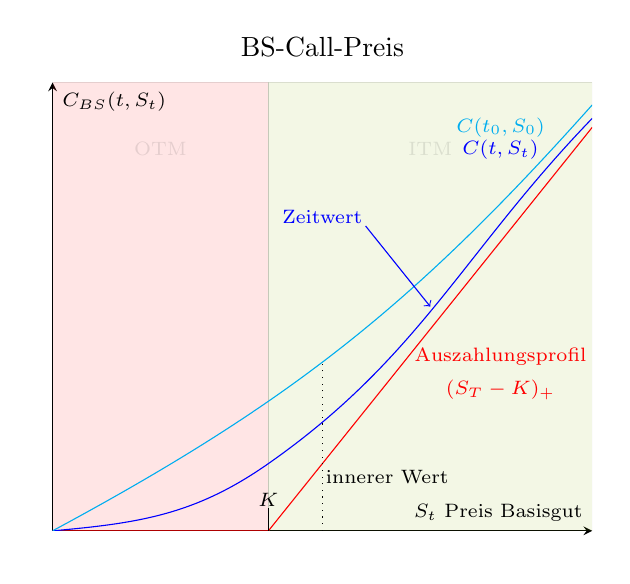
\begin{tikzpicture}
	\begin{axis}[
	xmin=0, xmax=1, xlabel=\scriptsize$S_t$ Preis Basisgut,
	ymin=0, ymax=1, ylabel={\scriptsize$C_{BS}(t,S_t)$},
	title=BS-Call-Preis,
	samples=400,
	axis x line=middle,
	axis y line=middle,
	domain=0:1,
	yticklabels={,,},
	xticklabels={,,},
	xtick style={draw=none},
	ytick style={draw=none},
	]
	\draw[fill=red,opacity=0.1] (axis cs: 0,0) rectangle (axis cs: 0.4,1) node[pos=0.5,black,yshift=2cm] {\scriptsize OTM};
	\draw[fill=lime!70!black,opacity=0.1] (axis cs: 0.4,0) rectangle (axis cs: 1,1) node[pos=0.5,black,yshift=2cm] {\scriptsize ITM};
	
	\draw[red] (axis cs: 0,0) -- (axis cs: 0.4,0) -- (axis cs: 1,0.9);
	\draw[blue] (axis cs: 0,0) to[out=5,in=215] (axis cs: 0.4,0.15) to[out=35,in=226] (axis cs: 1,0.92);
	\draw[cyan] (axis cs: 0,0) to[bend right=10] (axis cs: 1,0.95);
	
	\node[red,align=center] at (axis cs: 0.83,0.35) {\scriptsize Auszahlungsprofil\\\scriptsize$(S_T-K)_+$};
	\node[cyan] at (axis cs: 0.83,0.90) {\scriptsize $C(t_0,S_0)$};
	\node[blue] at (axis cs: 0.83,0.85) {\scriptsize $C(t,S_t)$};
	
	\draw (axis cs: 0.4,0) -- (axis cs: 0.4,0.05);
	\node at (axis cs: 0.4,0.07) {\scriptsize $K$};
	
	\draw[dotted] (axis cs: 0.5,0) -- (axis cs: 0.5,0.38);
	\node at (axis cs: 0.62,0.12) {\scriptsize innerer Wert};
	
	\node[blue] at (axis cs: 0.5,0.7) {\scriptsize Zeitwert};
	\draw[blue,->] (axis cs: 0.58,0.68) -- (axis cs: 0.7,0.5);
	\end{axis}
	\end{tikzpicture}
\end{center}
\begin{itemize}
	\item \begriff{innere Wert}: $(S_t -K)_+$ konvergiert gegen Auszahlungsprofil: $(S_T - K)_+$, für $t \to T$
	\item \begriff{Zeitwert}: $C_{BS}(t,S_t) - (S_t - K)_+ \ge 0$ konvergiert gegen Null für $t \to T$
	\item 
	\begin{itemize}
		\item \begriff{out of the money} (OTM): Innere Wert $=0$ bei $S_t < K$
		\item \begriff{in the money} (ITM): Innere Wert $>0$ bzw. $S_t > K$
		\item \begriff{at the money} (ATM): Grenzfall $S_t = K$
	\end{itemize}
	\item Zeitwert ist am größten für ATM-Optionen
	\item $t \mapsto C_{BS}(t,S_t)$ ist streng monoton fallend bzw.
	\begin{align*}
		\frac{\partial C_{BS}(t,S_t)}{\partial t} < 0
	\end{align*}
	\item $S_t \mapsto C_{BS}(t,S_t)$ ist streng monoton steigend und konvex bzw
	\begin{align*}
		\frac{\partial C_{BS}(t,S_t)}{\partial S}(t,S_t) > 0 \und \frac{\partial^2 C_{BS}}{\partial S^2}(t,S_t) > 0
	\end{align*}
	\item Für den Put ist das ganze Symmetrisch
\end{itemize}
Skizze vom BS-Put-Preis:
\begin{center}
	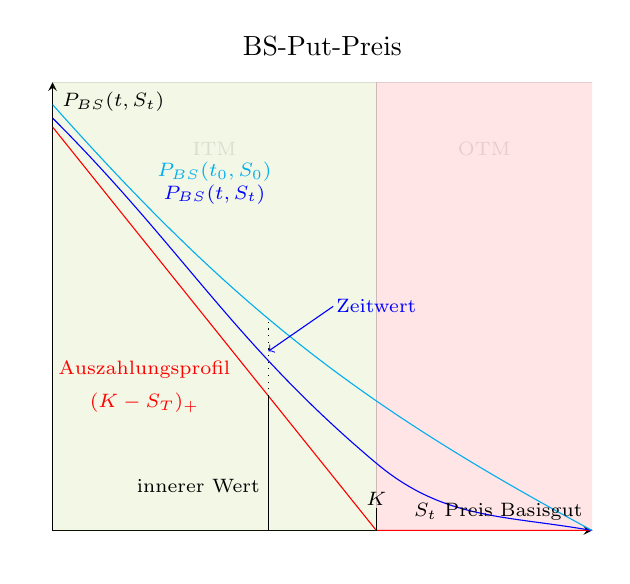
\begin{tikzpicture}
	\begin{axis}[
	xmin=0, xmax=1, xlabel=\scriptsize$S_t$ Preis Basisgut,
	ymin=0, ymax=1, ylabel={\scriptsize$P_{BS}(t,S_t)$},
	title=BS-Put-Preis,
	samples=400,
	axis x line=middle,
	axis y line=middle,
	domain=0:1,
	yticklabels={,,},
	xticklabels={,,},
	xtick style={draw=none},
	ytick style={draw=none},
	]
	\draw[fill=red,opacity=0.1] (axis cs: 0.6,0) rectangle (axis cs: 1,1) node[pos=0.5,black,yshift=2cm] {\scriptsize OTM};
	\draw[fill=lime!70!black,opacity=0.1] (axis cs: 0,0) rectangle (axis cs: 0.6,1) node[pos=0.5,black,yshift=2cm] {\scriptsize ITM};
	
	\draw[red] (axis cs: 0,0.9) -- (axis cs: 0.6,0) -- (axis cs: 1,0);
	\draw[blue] (axis cs: 0,0.92) to[out=-45,in=140] (axis cs: 0.6,0.15) to[out=-40,in=170] (axis cs: 1,0);
	\draw[cyan] (axis cs: 0,0.95) to[bend right=10] (axis cs: 1,0);
	
	\node[red,align=center] at (axis cs: 0.17,0.32) {\scriptsize Auszahlungsprofil\\\scriptsize$(K-S_T)_+$};
	\node[cyan] at (axis cs: 0.3,0.80) {\scriptsize $P_{BS}(t_0,S_0)$};
	\node[blue] at (axis cs: 0.3,0.75) {\scriptsize $P_{BS}(t,S_t)$};
	
	\draw (axis cs: 0.6,0) -- (axis cs: 0.6,0.05);
	\node at (axis cs: 0.6,0.07) {\scriptsize $K$};
	
	\draw (axis cs: 0.4,0) -- (axis cs: 0.4,0.3);
	\draw[dotted] (axis cs: 0.4,0.3) -- (axis cs: 0.4,0.47);
	\node at (axis cs: 0.27,0.1) {\scriptsize innerer Wert};
	
	\node[blue] at (axis cs: 0.6,0.5) {\scriptsize Zeitwert};
	\draw[blue,->] (axis cs: 0.52,0.5) -- (axis cs: 0.4,0.4);
	\end{axis}
	\end{tikzpicture}
\end{center}
\begin{itemize}
	\item \begriff{innere Wert}: $(K -S_t)_+$ konvergiert gegen Auszahlungsprofil: $(K - S_T)_+$, für $t \to T$
	\item \begriff{Zeitwert}: $P_{BS}(t,S_t) - (K - S_t)_+ \ge 0$ konvergiert gegen Null für $t \to T$
	\item 
	\begin{itemize}
		\item \begriff{out of the money} (OTM): Innere Wert $=0$ bei $S_t > K$
		\item \begriff{in the money} (ITM): Innere Wert $>0$ bzw. $S_t < K$
		\item \begriff{at the money} (ATM): Grenzfall $S_t = K$
	\end{itemize}
	\item Zeitwert ist am größten für ATM-Optionen
	\item $t \mapsto C_{BS}(t,S_t)$ ist streng monoton fallend bzw.
	\begin{align*}
	\frac{\partial C_{BS}(t,S_t)}{\partial t} < 0
	\end{align*}
	\item $S_t \mapsto C_{BS}(t,S_t)$ ist streng monoton fallend und konvex bzw
	\begin{align*}
	\frac{\partial C_{BS}(t,S_t)}{\partial S}(t,S_t) < 0 \und \frac{\partial^2 C_{BS}}{\partial S^2}(t,S_t) > 0
	\end{align*}
\end{itemize}
\begin{proof}[\propref{theo_BS_eq}]
	Wir beweisen das Resultat für $t = 0$: andere Zeitpunkte $t \in [0,T]$ können analog behandelt werden. 
	\begin{itemize}
		\item Nach \propref{theo_2_8}, gilt für Preis der Put-Option im $\CRR_N$-Modell
		\begin{align*}
		P^N(0, S_0^N) &= (1+r\Delta_n)^{-N}\cdot \E^{\QQ}[(K-S_T^N)_+]\\
		&= (1+r \Delta_n)^{-N}\cdot \E^{\QQ}[(K-S_0 e^{\ZZ_N = \log(\frac{S_T^N}{S_0})})]\\
		&= (1+ r \Delta_n)^{-N}\cdot \E^{\QQ}[f(\ZZ_N)]
		\end{align*}
		mit $f(z)= (K-S_0 e^z)_+$ stetig und beschränkt. Aus Stochastik ist bekannt $\ZZ_N \to \ZZ$ in Verteilung, dann folgt $\E[f(\ZZ_N)] \to \E[f(\ZZ)] \quad \forall f \in C_b(\R)$.
		\begin{itemize}
			\item $\lim_{N \to \infty}(1+r\Delta_n)^{-N} = \lim_{N \to \infty}(1+rT/N)^{-N} = e^{-rT}$
			\item $\lim_{N \to \infty} \E^{\QQ}[f(\ZZ_N)] = \E[f(Z)]$ mit $\ZZ \sim \NNN((r-\sigma^2/2)T, \sigma^2 T) = \NNN(mT,\sigma^2 T)$
			\begin{align*}
			\E[f(\ZZ)] &= \frac{1}{\sqrt{2\pi}}\frac{1}{\sigma\sqrt{T}}\int_{-\infty}^{\infty}(K-S_0 e^{\ZZ})_+ \exp(- \frac{(\ZZ - mt)^2}{2 \sigma^2 T})\d z\\
			&= \frac{1}{\sqrt{2 \pi}} \int_{-\infty}^{\log(K/S_0)}(K - S_0 e^{\ZZ})\exp(-\half (\frac{\ZZ-mT}{\sigma \sqrt{T}})^2) \d z\\
			&= \begin{pmatrix}
			y = \frac{\ZZ - mT}{\sigma \sqrt{T}}\\
			\d y = \frac{\d \ZZ}{\sigma \sqrt{T}}
			\end{pmatrix}\\
			&= \frac{1}{\sqrt{2 \pi}} \int_{-\infty}^{-d_2} (K - S_0 \exp(y \sigma \sqrt{T} + m T) e^{y^2/2} \d y\\
			&= K\Phi(-d_2)-S_0 \frac{1}{\sqrt{2 \pi}} \int_{-\infty}^{-d_2}\exp(-y^2/2 + y \sigma\sqrt{T}+mT)\d y
			\intertext{Nebenrechung:}
			& y^2/2 + y \sigma\sqrt{T} (+ mT = rT - \half(y^2-2y\sigma\sqrt{T}+\sigma^2 T) = rT - \half(y-\sigma\sqrt{T})\\
			&= K \Phi(-d_2) = S_0 e^{rT}\underbrace{\frac{1}{\sqrt{2 \pi}} \int_{-\infty}^{-d_2} e^{(y-\sigma\sqrt{T})/2}\d y}_{\Phi(-d_2-\sigma\sqrt{T})}\\
			&= K\Phi(-d_2) - S_0 e^{rT}\Phi(-d_1)\\
			\end{align*}
			Dann folgt $\lim_{N \to \infty} P_N(0, S_0^N) = e^{-rT}K\Phi(-d_2) - S_0\Phi(-d_1)$ und das ist die Formel für den Put \checkmark
		\end{itemize}
		\item Für Call: Nutze Put-Call-Parität
		\begin{align*}
			C^N(0,S_0) - \underbrace{P^N(0,S_0)}_{P_{BS}(0,S_0)} = \underbrace{S_0}_{S_0} - \underbrace{(1+ r\Delta_n)^{-N} K}_{\to e^{-rT}K}
		\end{align*} 
		\begin{align*}
			C_{BS}(0,S_0) &= \lim_{N \to \infty}C^N(0,S_0)\\
			&= P_{BS}(0,S_0) + S_0 - e^{rT}K\\
			&= e^{-rT}K(\underbrace{\Phi(-d_2)-1}_{-\Phi(d_2)}) - S_0 (\underbrace{\Phi(-d_1)-1}_{-\Phi(d_1)})\\
			&= S_0\Phi(d_1)-e^{-rT}K\Phi(d_2)
		\end{align*}
		wobei wir die Symmetrie der Normalverteilung: $\Phi(-x) = 1- \Phi(x)$ genutzt haben. Damit ist auch die BS-Formel für den Call gezeigt \checkmark.
	\end{itemize}
\end{proof}
\emph{Wir haben gezeigt:} $\CRR_N$-Preise konvergieren gegen BS-Preise.\\
\emph{Frage:} Was gilt für die Replikationsstrategie? Konvergiert diese auch?
\begin{theorem} %3.4
	Für die Replikationsstrategie $\xi_{t_N}^N$ der Put- bzw. Call-Optionen in $\CRR_N$-Modell gilt:
	\begin{itemize}
		\item \emph{Put:} $\lim_{N \to \infty} \xi_{t_N}^N = \frac{\partial P_{BS}}{\partial S}(t,S_t) = - \Phi(-d_1)$
		\item \emph{Call:} $\lim_{N \to \infty} \xi_{t_N}^N = \frac{\partial C_{BS}}{\partial S}(t,S_t) = \Phi(d_1)$
	\end{itemize}
	Diese partielle Ableitungen heißen auch ``Delta'' des Put- bzw. Call-Preisen. 
\end{theorem}
\begin{proof}
	Betrachte nur $t=0$, $t \in[0,T]$ kann analog behandelt werden. Nach \propref{th_2_3} ist $\xi_0^N$ für Put gegeben durch
	\begin{align*}
		\xi_0^N &= \frac{P_N(\Delta_N, S_0(1+b_N)) - P_N(\Delta_N, S_0(1+a_N))}{S_0(b_N-A_N)}\\
		&= \frac{P_N(\Delta_N, S_0(1+\mu\Delta_n + \sigma\sqrt{\Delta_n})) - P_N(\Delta_N, S_0(1+\mu\Delta_N + \sigma\sqrt{\Delta_N}))}{2 S_0 \sigma \sqrt{\Delta_N}}
	\end{align*}
	Es gilt $\lim_{N \to \infty} P_N(\Delta_N, S_0(1+\mu\Delta_N)) = P_{BS}(0,S_0)$. Unter geeigneten Annahmen an gleichmäßige Konvergenz folgt
	\begin{align*}
		\lim_{N \to \infty} \xi_0^N = \frac{\partial P_{BS}}{\partial S}(t,S_t)
	\end{align*}
	und analog für Call. Wir berechnen explizit:
	\begin{align*}
		\frac{\partial C_{BS}}{\partial S}(t,S) &= \Phi(d_1) + S\phi(d_1)\cdot \frac{\partial d_1}{\partial S} - e^{-r(T-t)}K\phi(d_2)\frac{\partial d_2}{\partial S}\\
		&= \Phi(d_1) + \frac{\partial d_1}{\partial S}(S\phi(d_1)-e^{-r(T-t)}K\phi(d_2))
		\intertext{Nebenrechung:}
		e^{-rt}K/S\phi(d_2) &= e^{-r\tau}\frac{1}{\sqrt{2\pi}}K/S \exp(-\half \frac{\log(S/K) + r\tau - \sigma^2 r/\tau}{\sigma \sqrt{\tau}})\\
		&= \frac{1}{\sqrt{2\pi}} e^{-r\tau}K/S \exp(-\half \frac{(\log(S/K) + r\tau)^2}{\sigma^2 \tau} - 2 (\log(S/K) + r\tau) + \sigma^2\tau/4)\\
		&= \frac{1}{\sqrt{2\pi}}\exp(-\half \frac{(\log(S/K) + r\tau)^2}{\sigma^2 \tau} + (\log(S/K) + r \tau + \sigma^2\tau/4)\\
		&= \phi(d_1)
	\end{align*}
	also 
	\begin{align*}
		e^{-r(T-t)}K \phi(d_2) = S\phi(d_1)
	\end{align*}
	Das heißt: $\frac{\partial C_{BS}}{\partial S}(t,S) = \Phi(d_1)$. Put folgt analog oder mit Put-Call-Parität.
\end{proof}
\begin{*remark}
	\begin{itemize}
		\item $\frac{\partial C_{BS}}{\partial S}$ bzw. $\frac{\partial P_{BS}}{\partial S}$ lassen sich auch interpretieren als \begriff{Sensitivität} des Call- bzw. Put-Preises gegenüber Preisänderungen des Basisguts.
	\end{itemize}
\end{*remark}
Analog lassen sich die Sensitivitäten (``\begriff{Greeks}'') nach den weiteren Parametern berechnen.
\begin{definition}
	Die ``Greeks'' des BS-Preises sind folgende partielle Ableitungen\\
	\begin{tabular}{|c|c|c|c|c|} % TODO fix the table :/
		Bezeichg. & part. Abl. & Call & Put & Bemerkungen\\
		\hline
		Delta & $\frac{\partial}{\partial S}$ & $\Phi(d_1)$ & $-\Phi(-d_1)$ & Bestimmt die Replikations- bzw. Hedgingstrat.\\
		Gamma & $\frac{\partial^2}{\partial S^2}$ & $\frac{\phi(d_1)}{S\sigma\sqrt{T-t}}$ & $\frac{\phi(d_1)}{S\sigma\sqrt{T-t}}$ & Sensitivität von Delta ggü Basisgut, ``wie oft'' muss Strategie anpassen: Konvexität\\
		Vega & $\frac{\partial}{\partial \sigma}$ & $S_t \sqrt{T-t}\phi(d_1)$ & $S_t \sqrt{T-t}\phi(d_1)$ & Sensitivität gegenüber Änderg Volatitität ($\nu >0$)\\
		Theta & $\frac{\partial}{\partial t}$ & siehe ÜA & siehe ÜA & Änderung in der Zeit\\
		Rho & $\frac{\partial}{\partial r}$ & $K(T-t)(e^{-r(T-t)}) \Phi(d_2)$ & $-K(T-t)(e^{-r(T-t)}) \Phi(-d_2)$ & Sensitivität ggü Änderung Zinsrate
	\end{tabular}
\end{definition}
\begin{*remark}
	``Vega'' ist kein Buchstabe des griechischen Alphabets :/
\end{*remark}
\begin{conclusion}
	Der BS-Preis $C_{BS}(t,S)$ erfüllt folgende partielle DGL
	\begin{align*}
		\frac{\partial C_{BS}}{\partial t} + rS\frac{\partial C_{BS}}{\partial S} + \frac{\sigma^2}{2}S^2 \frac{\partial^2 C_{BS}}{\partial S^2}+rC_{BS} = 0 \tag{BS-PDE}\label{eq_3_1_BS_PDE}
	\end{align*}
	wobei $(t,s) \in [0,T]\times \R_{\ge 0}$. Mit Endwertbedingung
	\begin{align*}
		\lim_{t \to T} C_{BS}(t,S) = (S-K)_+
	\end{align*}
	Für $P_{BS}$ gilt die gleiche PDE mit Endwertbedingung
	\begin{align*}
		\lim_{t \to T} P_{BS}(t,S) = (K-S)_+
	\end{align*}
\end{conclusion}
\begin{proof}
	Siehe Übung 3.0.
\end{proof}
\begin{*remark}
	In Erweiterungen des BS-Modells gibt es \emph{keine} geschlossene Ausdrücke für Put/Call-Preise, aber eine PDE ähnlich zu \eqref{eq_3_1_BS_PDE} gilt weiterhin.
\end{*remark}
\section{Implizite Volatilität/ Grenzen des BS-Modells}
Wir schreiben etwas ausführlicher
\begin{align*}
	C_{BS}(t,S_t, T, K, \sigma) := C_{BS}(t, S_t)
\end{align*}
eine Abhängigkeit von $(T,K,\sigma)$ zu verdeutlichen.
\begin{theorem}[Implizite Volatlität] %3.6
	Sei $C_{\ast}(0,S_0,T, K)$ ein vorgegebener (beobachtbarer) Preis einer Call-Option mit Fälligkeit $T$, Ausübungspreis $K$ welcher innerhalb der Arbitragegrenzen liegt
	\begin{align*}
		(S_0 - e^{-rT}K)_+ < C_{\ast}(0,S_0, T,K) < S_0
	\end{align*}
	Dann existiert ein eindeutiges $\sigma_{\ast}(T, K) \in (0,\infty)$, die \begriff{implizite Volativilität} von $C_{\ast}$ sodass
	\begin{align*}
		C_{\ast}(0,S_0, T,K) = C_{BS}(0,S_0,T,K, \sigma_{\ast}(T,K))
	\end{align*}
	gilt.
\end{theorem}
\begin{*remark}
	$\sigma_{\ast}(T,K)$ ist Lösung eines inversen Problems.
	\begin{align*}
		\begin{matrix}
			\text{Vorwärtsproblem: } & \text{ Parameter }\to \text{ Call-Preis}\\
			\text{inverses Problem: } & \text{ Call-Preis }\to \text{ Parameter}
		\end{matrix}
	\end{align*}
	Kann zur impirischen Überpürfung des BS-Modells verwendet werden:
	\begin{itemize}
		\item BS-Modell passt gut zu Daten: $(T,K) \mapsto \sigma_{\ast}(T,K)$ ist annähernd konstant
		\item BS-Modell passt nicht gut zu Daten: $(T,K) \mapsto \sigma_{\ast}(T,K)$ variiert stark mit $(T,K)$
	\end{itemize}
\end{*remark}
Typische tatsächliche Beobachtung:\\
\begin{center}
	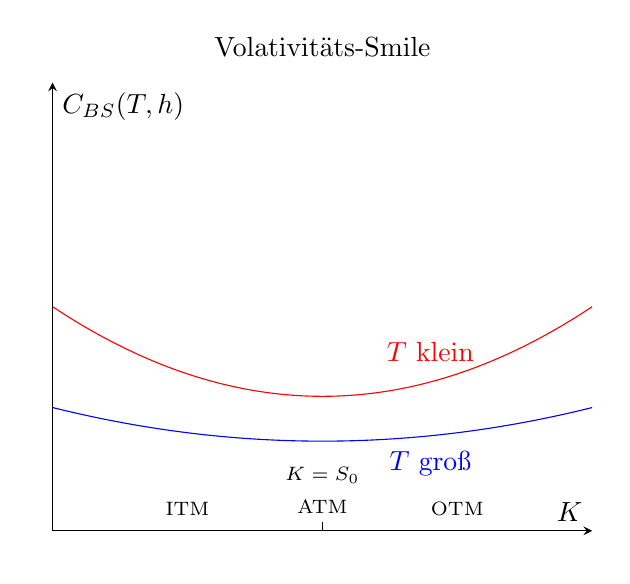
\begin{tikzpicture}
	\begin{axis}[
	xmin=0, xmax=1, xlabel=$K$,
	ymin=0, ymax=1, ylabel={$C_{BS}(T,h)$},
	title=Volativitäts-Smile,
	samples=400,
	axis x line=middle,
	axis y line=middle,
	domain=0:1,
	yticklabels={,,},
	xticklabels={,,},
	xtick style={draw=none},
	ytick style={draw=none},
	]
	\addplot[mark=none,smooth,blue] {0.3*(x-0.5)*(x-0.5)+0.2};
	\addplot[mark=none,smooth,red] {0.8*(x-0.5)*(x-0.5)+0.3};
	\node[blue] at (axis cs: 0.7,0.15) {$T$ groß};
	\node[red] at (axis cs: 0.7,0.4) {$T$ klein};
	
	\draw (axis cs: 0.5,0) -- (axis cs: 0.5,0.02);
	\node[align=center] at (axis cs: 0.5,0.09) {\scriptsize$K=S_0$\\ \scriptsize ATM};
	\node[align=center] at (axis cs: 0.25,0.05) {\scriptsize ITM};
	\node[align=center] at (axis cs: 0.75,0.05) {\scriptsize OTM};
	\end{axis}
	\end{tikzpicture}
\end{center}
Eigenschaften:
\begin{itemize}
	\item konvex
	\item assymetrisch (höher für große K)
	\item Minimum bei ATM
	\item flacher für lange Laufzeiten, steiler für kurze Laufzeiten
\end{itemize}
Form weist daraufhin, dass BS-Modell große Preissprünge des Basisguts \emph{unterschätzt}. Form des \person{Vola}-\person{Smiles} in Modellen jeweils von BS $\implies$ \emph{aktuelles Forschungsthema}.